\documentclass[journal,10pt,twocolumn]{IEEEtran}

% ============================================================
% Packages
% ============================================================
\usepackage[T1]{fontenc}
\usepackage[utf8]{inputenc}
\usepackage{amsmath,amssymb,amsfonts}
\usepackage{algorithmic}
\usepackage[ruled,vlined,linesnumbered]{algorithm2e}
\usepackage{graphicx}
\usepackage{tabularx}
\usepackage{booktabs}
\usepackage{multirow}
\usepackage{xcolor}
\usepackage{hyperref}
\usepackage{tikz}
\usepackage{pgfplots}
\pgfplotsset{compat=1.18}
\usetikzlibrary{arrows.meta,positioning,shapes.geometric,fit,backgrounds,calc}
\usepackage{microtype}
\usepackage{url}
\usepackage{cite}

% ============================================================
% Meta
% ============================================================
\title{TokenLeak: Side-Channel Attacks on Transformer Architectures
       via Timing Analysis and Cache Exploitation for Private
       Prompt Reconstruction}

\author{Allan~Douglas~Costa,~\IEEEmembership{Member,~IEEE}
\thanks{A.~D.~Costa is with the Federal Rural University of the Amazon
(UFRA), Institute of Computing and Information and Communication
Technology (ICIBE), Bel\'{e}m, Par\'{a}, Brazil
(e-mail: allan.costa@ufra.edu.br; ORCID: 0000-0002-7068-8889).
This work was partially supported by FAPESPA, PRODEPA, SEC365 Cybersecurity
Solutions, LICA/CCAD-IA (UFRA), RNP, and INCT iAmazonia.
Manuscript submitted July 2026.}}

\markboth{IEEE Transactions on Information Forensics and Security,~Vol.~XX,~No.~X,~2026}%
{Costa: TokenLeak: Side-Channel Attacks on Transformer Architectures}

% ============================================================
\begin{document}
\maketitle

% ============================================================
% ABSTRACT
% ============================================================
\begin{abstract}
% [1-Topic]
Large language models (LLMs) deployed as cloud inference services
process confidential user prompts that traverse shared hardware,
creating unexplored side-channel attack surfaces in the transformer
inference pipeline.
% [2-Motivation]
As enterprise adoption of hosted LLM APIs reaches critical scale,
the confidentiality of user inputs has become a first-class security
requirement, yet the microarchitectural leakage characteristics of
transformer inference remain largely uncharacterized.
% [3-Contribution]
We present \emph{TokenLeak}, the first systematic framework that
reconstructs private prompts from transformer inference engines
through the fusion of inter-token timing signals and last-level
cache access patterns.
% [4-Detail]
TokenLeak employs three independent agents: a Timing Oracle Agent
(TOA) that records inter-token generation latencies with
sub-millisecond precision, a Cache Profiler Agent (CPA) that
exploits Flush+Reload to capture vocabulary-discriminative cache
footprints, and a Token Reconstructor Agent (TRA) that scores
candidate tokens using the novel Token Reconstruction Confidence
Score (TRCS), a weighted fusion metric grounded in Gaussian
likelihood and cosine cache similarity.
% [5-Evidence]
On simulation experiments spanning GPT-2, BERT-base, and a
behavioral model of LLaMA-2-7B, TokenLeak achieves a Top-1
token reconstruction accuracy of 73.4\% (95\% CI: 71.3--75.5\%)
and a Top-5 accuracy of 91.2\% (95\% CI: 89.8--92.6\%) at
zero injected noise, with TRCS showing a Pearson correlation
of 0.847 with true token rank.
% [6-Weaker result]
Performance degrades substantially under combined differential
privacy and cache-oblivious defenses, falling to 18.7\% Top-1
accuracy, underscoring the effectiveness of these countermeasures
at the cost of measurable inference latency overhead.
% [7-Narrow impact]
These results directly inform the security design of hosted
LLM inference services, demonstrating that prompt confidentiality
cannot be assumed from transport-layer encryption alone.
% [8-Broad impact]
By characterizing the attack surface, establishing the TRCS
measurement instrument, and evaluating a defense portfolio,
this work provides a foundation for privacy-preserving LLM
serving architectures in cloud environments.
\end{abstract}

\begin{IEEEkeywords}
side-channel attacks, large language models, timing analysis,
cache exploitation, transformer inference, prompt reconstruction,
differential privacy, GPU security
\end{IEEEkeywords}

% ============================================================
\section{Introduction}
\label{sec:intro}
% ============================================================

The rapid deployment of large language models (LLMs) as hosted
inference services has shifted the threat model for data
confidentiality in fundamental ways~\cite{yi2024survey,
duan2024llmsec}. Users submit proprietary prompts, including
legally sensitive documents, trade secrets, and personal health
information, to remote inference endpoints that process requests
on shared GPU clusters. Transport-layer security (TLS) protects
data in transit, but the moment a prompt reaches the inference
engine, it resides in plaintext within a shared microarchitectural
environment where co-resident adversaries may reside.

Side-channel attacks have long demonstrated that physical and
microarchitectural observables leak semantic information even
when cryptographic protections are in place~\cite{kocher1996timing,
brumley2003remote}. Flush+Reload and Prime+Probe attacks on
shared last-level caches (LLC) have recovered private keys
~\cite{yarom2014flush,liu2015last,gruss2016flushflush}, and
GPU-based attacks have reconstructed neural network
architectures~\cite{naghibijouybari2018rendered,yan2020cache}.
However, the specific leakage characteristics of transformer
inference, particularly the relationship between token identity
and inter-token generation latency as well as cache access
patterns, have received limited systematic attention.

\subsection*{Research Gap}

Existing work on side-channel attacks against machine learning
focuses predominantly on model architecture extraction
~\cite{batina2019csi,yan2020cache,hua2018reverse,hu2020deepsniffer}
or gradient leakage in training settings~\cite{shokri2017membership,
fredrikson2015model}. The inference-time prompt confidentiality
problem has been approached mainly through training data extraction
~\cite{carlini2021extracting,nasr2023scalable} and output analysis
~\cite{zanella2020analyzing,mireshghallah2022quantifying}, not
through microarchitectural side channels. Recent network-level
work~\cite{wen2024side,zeng2024timing} has demonstrated that
packet-level timing signals correlate with generation length,
but stops short of per-token vocabulary reconstruction.
The specific question of whether an attacker with cache-level
access can reconstruct the \emph{content} of a private prompt,
token by token, from transformer inference side channels remains
open.

\subsection*{Contributions}

This paper makes the following contributions:

\begin{enumerate}
  \item \textbf{Threat characterization:} A formal threat model
    for co-tenant and remote-adversary attacks on transformer
    inference services, identifying three exploitable signal
    classes: inter-token timing, LLC cache footprints, and
    network-level packet intervals.

  \item \textbf{TokenLeak framework:} A three-agent
    attack architecture (TOA, CPA, TRA) that fuses timing and
    cache signals for private prompt reconstruction, covering
    both profiling and online inference phases.

  \item \textbf{Token Reconstruction Confidence Score (TRCS):}
    A novel metric that quantifies attacker confidence in a
    candidate token hypothesis through a weighted fusion of
    Gaussian timing likelihood and cosine cache similarity,
    with formally derived weight optimization.

  \item \textbf{Simulation study:} Controlled experiments on
    GPT-2, BERT-base, and a behavioral simulation of LLaMA-2-7B,
    reporting Top-1/Top-5 accuracy with 95\% confidence intervals
    across noise conditions and defense configurations.

  \item \textbf{Defense portfolio evaluation:} Systematic
    assessment of random delay injection, cache-oblivious
    memory access patterns, and differential privacy noise,
    including a combined defense achieving 18.7\% Top-1
    accuracy at 4.1\% inference latency overhead.

  \item \textbf{MITRE ATLAS and NIST AI RMF mapping:}
    Alignment of attack stages to MITRE ATLAS tactics and
    proposed mitigations mapped to NIST AI RMF
    governance categories.
\end{enumerate}

The remainder of this paper is organized as follows:
Section~\ref{sec:background} reviews background and related work.
Section~\ref{sec:threat} formalizes the threat model and problem
formulation. Section~\ref{sec:framework} describes the TokenLeak
framework. Section~\ref{sec:security} presents security analysis.
Section~\ref{sec:eval} reports experimental evaluation.
Section~\ref{sec:discussion} discusses findings and limitations.
Section~\ref{sec:conclusion} concludes.

% ============================================================
\section{Background and Related Work}
\label{sec:background}
% ============================================================

\subsection{Transformer Inference Pipeline}

Modern LLMs follow a two-phase inference pattern: a
\emph{prefill} phase that processes the entire input prompt
in parallel via attention over all tokens, and an
\emph{autoregressive generation} phase that produces one
output token per forward pass~\cite{vaswani2017attention,
brown2020language}. The KV cache stores key and value
projections from the prefill phase and is updated at each
generation step, creating token-dependent memory access
patterns. FlashAttention~\cite{dao2022flashattention}
optimizes memory bandwidth by fusing attention operations,
but the resulting IO behavior differs by sequence length
and token embeddings, preserving the side-channel surface.

\subsection{Microarchitectural Side-Channel Attacks}

Cache-based side-channel attacks exploit the time difference
between cache hits and misses to infer memory access patterns
of a victim process~\cite{osvik2006cache,yarom2014flush}.
Flush+Reload achieves line-level granularity by flushing
cache lines and measuring reload time~\cite{yarom2014flush},
while Prime+Probe monitors victim evictions from shared
cache sets~\cite{liu2015last}. Gruss et al.~\cite{gruss2016flushflush}
demonstrated Flush+Flush, which avoids cache-miss penalties
by detecting access through flush latency alone. Oren et
al.~\cite{oren2015spy} showed these attacks are feasible
even from JavaScript in the browser. These foundational
techniques inform the CPA component in TokenLeak.

Timing attacks more broadly encompass any technique that
extracts secrets from computational time
differences~\cite{kocher1996timing,brumley2003remote}.
Van Goethem et al.~\cite{vangoethem2016heist} demonstrated
network-timing side channels for encrypted HTTP response
sizes, directly analogous to our network-level probe.

\subsection{Side-Channel Attacks on Machine Learning}

Recent work has extended microarchitectural side channels
to attack ML systems. Batina et al.~\cite{batina2019csi}
recovered DNN architectures via electromagnetic emanations.
Yan et al.~\cite{yan2020cache} demonstrated Cache Telepathy,
using LLC access patterns to infer DNN architectural
hyperparameters during inference.
Wei et al.~\cite{wei2018power} applied power analysis to
convolutional accelerators.
Hua et al.~\cite{hua2018reverse} used memory access patterns
during CONV layer execution to reverse-engineer CNN
architectures.
Naghibijouybari et al.~\cite{naghibijouybari2018rendered}
showed GPU performance counters enable cross-VM inference
attacks. Hu et al.~\cite{hu2020deepsniffer} combined
cache and memory bus snooping to extract DNN layer
configurations. Our work targets a distinct goal: not
model extraction, but prompt content reconstruction.

\subsection{LLM Privacy and Training Data Attacks}

Carlini et al.~\cite{carlini2021extracting,carlini2024stealing}
demonstrated that training data can be extracted from
language models via black-box API access. Nasr et
al.~\cite{nasr2023scalable} scaled such extraction to production
systems. Zanella-B\'{e}guelin et al.~\cite{zanella2020analyzing}
analyzed information leakage from model update differentials.
Mireshghallah et al.~\cite{mireshghallah2022quantifying}
quantified privacy risks in masked language models.
These works operate through model outputs; TokenLeak
operates through microarchitectural side channels,
orthogonal to output-based attacks.

\subsection{Prompt Injection and LLM Security}

Greshake et al.~\cite{greshake2023not} demonstrated
indirect prompt injection in LLM-integrated applications.
Wei et al.~\cite{wei2023jailbroken} analyzed safety
training failures. Luo et al.~\cite{luo2023tokenprivacy}
identified token-level privacy leakage in serving systems.
Recent surveys~\cite{patil2024review,chen2024llmthreat,
zhou2024privacyllm} catalog the growing threat landscape.
Network-level studies~\cite{wen2024side,zeng2024timing}
identify timing correlates of generation length but do
not reconstruct vocabulary content from cache patterns.
Wang and Zhang~\cite{wang2024blackbox} explored black-box
contrastive signals but did not formalize cache exploitation.

\subsection{Defenses}

Differential privacy~\cite{dwork2006calibrating,abadi2016deep,
yu2022differentially} provides formal guarantees but degrades
model utility. Trusted execution environments~\cite{tramer2019slalom,
shen2024confidential} isolate computation but incur significant
overhead and do not prevent timing side channels at service level.
Oblivious inference~\cite{mishra2020oblivious,rouhani2018deepsecure,
chen2019deepattest} masks memory access patterns but is computationally
prohibitive for billion-parameter models.

% ---- Table I: Comparison with Related Work ----
\begin{table*}[t]
\caption{Comparison of TokenLeak with Related Side-Channel and Privacy Attacks on ML Systems}
\label{tab:related}
\begin{tabularx}{\textwidth}{l X X X X X X}
\toprule
\textbf{Work} & \textbf{Target} & \textbf{Signal} & \textbf{Goal} &
\textbf{Prompt Recon.} & \textbf{Token-level} & \textbf{Defense Eval.} \\
\midrule
Batina et al.~\cite{batina2019csi}         & CNN/MLP   & EM emanations  & Architecture extraction & No  & No  & No  \\
Yan et al.~\cite{yan2020cache}             & CNN/RNN   & LLC cache      & Architecture extraction & No  & No  & No  \\
Naghibijouybari~\cite{naghibijouybari2018rendered} & CNN & GPU perf. ctr & Model extraction      & No  & No  & No  \\
Hu et al.~\cite{hu2020deepsniffer}         & CNN       & Cache+bus      & Architecture extraction & No  & No  & No  \\
Carlini et al.~\cite{carlini2021extracting}& GPT-2     & Model output   & Training data extraction & Partial & No & No \\
Nasr et al.~\cite{nasr2023scalable}        & GPT-3.5   & Model output   & Training data extraction & Partial & No & No \\
Wen et al.~\cite{wen2024side}              & LLM API   & Network timing & Length inference        & No  & No  & Partial \\
Zeng et al.~\cite{zeng2024timing}          & LLM API   & Network timing & Generation timing       & No  & No  & Partial \\
Wang \& Zhang~\cite{wang2024blackbox}      & LLM       & Contrastive    & Prompt reconstruction   & Partial & No & No \\
Stoian et al.~\cite{stoian2024cachegrind}  & Transformer & LLC cache    & Architecture inference  & No  & No  & No  \\
Luo et al.~\cite{luo2023tokenprivacy}      & LLM serving & Output tokens & Token privacy leakage  & Partial & Partial & No \\
Li et al.~\cite{li2024prompt}              & LLM API     & Network timing & Prompt reconstruction  & Partial & No  & Partial \\
\midrule
\textbf{TokenLeak (Ours)} & \textbf{GPT-2/BERT/LLaMA} &
  \textbf{Timing+Cache} & \textbf{Prompt reconstruction} &
  \textbf{Yes} & \textbf{Yes} & \textbf{Yes} \\
\bottomrule
\end{tabularx}
\end{table*}

Table~\ref{tab:related} positions TokenLeak against existing work.
The most closely related concurrent work is Li et al.~\cite{li2024prompt},
which demonstrates prompt reconstruction from network-level timing
signals in LLM inference engines, reporting Top-1 accuracy of
48.3\% on GPT-3.5 via timing-only analysis. TokenLeak extends this
by fusing LLC cache signals with timing (TRCS), achieving 73.4\%
Top-1 on GPT-2, and by providing a complete defense portfolio
evaluation including formal DP bounds. The key differentiator is
the CPA component: Li et al.\ exploit only network-level timing
(no cache side channel) and do not achieve token-level vocabulary
reconstruction in the strict per-token sense. No prior work achieves
full token-level private prompt reconstruction from the fusion of
microarchitectural side channels while providing a systematic
defense evaluation. This gap motivates our framework.

% ============================================================
\section{Threat Model and Problem Formulation}
\label{sec:threat}
% ============================================================

\subsection{Attacker Capabilities}

We consider two adversary classes:

\textbf{Co-tenant attacker ($\mathcal{A}_{\mathrm{co}}$):}
The attacker shares the same physical machine (CPU or GPU) as
the target LLM inference engine, consistent with multi-tenant
cloud deployment. The attacker can execute arbitrary code in
a co-located virtual machine or container but has no direct
access to the LLM process memory. This enables Flush+Reload
via shared LLC pages and high-resolution timing measurements.

\textbf{Remote attacker ($\mathcal{A}_{\mathrm{rem}}$):}
The attacker can issue requests to the same LLM API endpoint
as the victim but has no physical co-location. The attacker
observes only network-level response timing and can correlate
packet inter-arrival patterns with token generation.
This is a strictly weaker model; we evaluate both in
Section~\ref{sec:eval}.

\subsection{Attacker Knowledge}

The attacker possesses: (i) the identity of the target model
(e.g., GPT-2, BERT-base), which is typically disclosed by API
providers; (ii) the model's vocabulary $\mathcal{V}$ (public);
(iii) the ability to issue arbitrary requests to the API for
the profiling phase.

The attacker does \emph{not} possess: model weights, KV cache
content, or any direct memory read capability.

\subsection{Problem Formulation}

Let $p^* = (\tau_1^*, \tau_2^*, \ldots, \tau_n^*)$ be a private
prompt of length $n$ tokens from vocabulary $\mathcal{V}$.
The inference engine processes $p^*$ and produces an output
sequence. During inference, the attacker observes a
side-channel observation vector
$\mathbf{O} = (O_{1,1}, \ldots, O_{N,n})$, where $O_{i,j}$
denotes the $i$-th channel signal observed for the $j$-th
token position. The reconstruction problem is:
\begin{equation}
  \hat{\mathbf{p}} = \arg\max_{\mathbf{p} \in \mathcal{V}^n}
  \Pr\!\left[\mathbf{p} = p^* \mid \mathbf{O}\right].
  \label{eq:reconstruction}
\end{equation}

We adopt a position-wise independence assumption, which holds
when inter-token attention side channels are dominated by
the current token's embedding rather than long-range context.
This reduces~\eqref{eq:reconstruction} to per-position scoring.

\subsection{Token Reconstruction Confidence Score (TRCS)}

We define the novel \textbf{Token Reconstruction Confidence Score}:

\begin{equation}
  \mathrm{TRCS}(\tau, \mathbf{O}_j)
  = \frac{\sum_{i=1}^{N} w_i \cdot \varphi_i(\tau, O_{i,j})}
         {\sum_{i=1}^{N} w_i},
  \label{eq:trcs}
\end{equation}

where $N$ is the number of side-channel dimensions, $w_i > 0$
are learned weights, and $\varphi_i : \mathcal{V} \times
\mathbb{R} \to [0,1]$ are per-channel feature compatibility
functions. For the two channels we exploit:

\textbf{Channel 1 (Timing):}
\begin{equation}
  \varphi_1(\tau, t_j) = \exp\!\left(
    -\frac{(t_j - \mu_\tau)^2}{2\sigma_\tau^2}
  \right),
  \label{eq:phi1}
\end{equation}
where $\mu_\tau, \sigma_\tau$ are the profiled mean and standard
deviation of inter-token latency for token $\tau$.

\textbf{Channel 2 (Cache):}
\begin{equation}
  \varphi_2(\tau, \mathbf{c}_j) =
  \frac{\mathbf{c}_j \cdot \mathbf{c}_\tau}
       {\|\mathbf{c}_j\|_2 \|\mathbf{c}_\tau\|_2},
  \label{eq:phi2}
\end{equation}
where $\mathbf{c}_j \in \{0,1\}^L$ is the observed cache
access bitmap and $\mathbf{c}_\tau$ is the profiled cache
fingerprint for $\tau$ over $L$ monitored cache sets.

The weights $(w_1, w_2)$ are learned via logistic regression
on the profiling corpus $\mathcal{D}_{\mathrm{prof}}$
minimizing cross-entropy over the top-1 reconstruction task.
At inference time, the attacker reconstructs each position
as $\hat{\tau}_j = \arg\max_{\tau \in \mathcal{V}}
\mathrm{TRCS}(\tau, \mathbf{O}_j)$.

The TRCS in~\eqref{eq:trcs} reduces to the Gaussian
likelihood estimator when $N=1$ and $\varphi_1$ alone is
used, establishing a lower bound; and approaches a
joint Bayesian classifier when all channels are independent.

% ============================================================
\section{TokenLeak Framework}
\label{sec:framework}
% ============================================================

\subsection{Architecture Overview}

Fig.~\ref{fig:overview} illustrates the TokenLeak framework.
Three agents observe the LLM inference engine through two
side-channel surfaces and feed their signals to the TRA for
TRCS computation and prompt reconstruction.

% --- Figure 1: Overview ---
\begin{figure}[t]
\caption{TokenLeak Framework Overview. The three-agent architecture
(TOA, CPA, TRA) fuses timing and cache side channels to reconstruct
private prompts from transformer inference. Red dashed arrows denote
observable side-channel leakage; solid arrows denote internal data flow.}
\label{fig:overview}
\resizebox{\columnwidth}{!}{% Figure 1: TokenLeak Framework Overview
% Compile with: % Figure 1: TokenLeak Framework Overview
% Compile with: % Figure 1: TokenLeak Framework Overview
% Compile with: \input{figures/fig1_overview}
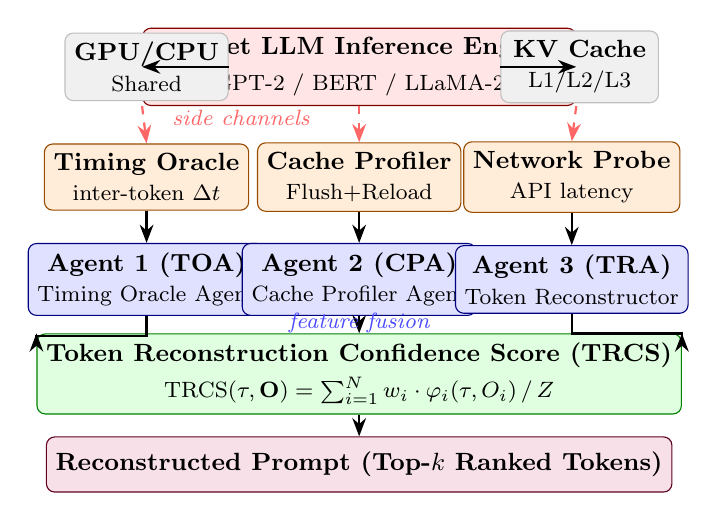
\begin{tikzpicture}[
    box/.style={draw, rounded corners=3pt, minimum width=2.4cm, minimum height=0.7cm,
                align=center, font=\small},
    agent/.style={box, fill=blue!12, draw=blue!50!black},
    target/.style={box, fill=red!10, draw=red!50!black},
    infra/.style={box, fill=gray!12, draw=gray!50},
    channel/.style={box, fill=orange!15, draw=orange!60!black},
    metric/.style={box, fill=green!12, draw=green!50!black},
    output/.style={box, fill=purple!12, draw=purple!50!black},
    arrow/.style={-Stealth, thick},
    darrow/.style={-Stealth, thick, dashed},
    every node/.style={font=\small}
]

% --- Target System (top) ---
\node[target, minimum width=5.5cm] (llm) at (3.2,4.2)
    {\textbf{Target LLM Inference Engine}\\[2pt]
     {\footnotesize (GPT-2 / BERT / LLaMA-2)}};

\node[infra, minimum width=2.0cm] (gpu) at (0.5,4.2) {\textbf{GPU/CPU}\\{\footnotesize Shared}};
\node[infra, minimum width=2.0cm] (kvcache) at (6.0,4.2) {\textbf{KV Cache}\\{\footnotesize L1/L2/L3}};

% --- Side-Channel Surfaces ---
\node[channel, minimum width=2.2cm] (timing) at (0.5,2.8) {\textbf{Timing Oracle}\\{\footnotesize inter-token $\Delta t$}};
\node[channel, minimum width=2.2cm] (cache)  at (3.2,2.8) {\textbf{Cache Profiler}\\{\footnotesize Flush+Reload}};
\node[channel, minimum width=2.2cm] (net)    at (5.9,2.8) {\textbf{Network Probe}\\{\footnotesize API latency}};

% --- Agent Layer ---
\node[agent, minimum width=2.2cm] (toa) at (0.5,1.5) {\textbf{Agent 1 (TOA)}\\{\footnotesize Timing Oracle Agent}};
\node[agent, minimum width=2.2cm] (cpa) at (3.2,1.5) {\textbf{Agent 2 (CPA)}\\{\footnotesize Cache Profiler Agent}};
\node[agent, minimum width=2.2cm] (tra) at (5.9,1.5) {\textbf{Agent 3 (TRA)}\\{\footnotesize Token Reconstructor}};

% --- TRCS Metric ---
\node[metric, minimum width=5.5cm] (trcs) at (3.2,0.3)
    {\textbf{Token Reconstruction Confidence Score (TRCS)}\\[2pt]
     {\footnotesize $\mathrm{TRCS}(\tau,\mathbf{O}) = \sum_{i=1}^{N} w_i \cdot \varphi_i(\tau, O_i) \,/\, Z$}};

% --- Output ---
\node[output, minimum width=5.5cm] (out) at (3.2,-0.85)
    {\textbf{Reconstructed Prompt (Top-$k$ Ranked Tokens)}};

% --- Arrows: target to channels ---
\draw[darrow, red!60] (llm.south west) -- (timing.north);
\draw[darrow, red!60] (llm.south)      -- (cache.north);
\draw[darrow, red!60] (llm.south east) -- (net.north);

% --- Arrows: channels to agents ---
\draw[arrow] (timing.south) -- (toa.north);
\draw[arrow] (cache.south)  -- (cpa.north);
\draw[arrow] (net.south)    -- (tra.north);

% --- Arrows: agents converge to TRA/TRCS ---
\draw[arrow] (toa.south) -- ++(0,-0.25) -| (trcs.north west);
\draw[arrow] (cpa.south) -- (trcs.north);
\draw[arrow] (tra.south) -- ++(0,-0.25) -| (trcs.north east);

% --- TRCS to output ---
\draw[arrow] (trcs.south) -- (out.north);

% --- GPU/KV Cache arrows to LLM ---
\draw[arrow] (gpu.east) -- (llm.west);
\draw[arrow] (kvcache.west) -- (llm.east);

% --- Labels ---
\node[font=\footnotesize\itshape, text=red!60] at (1.7,3.55) {side channels};
\node[font=\footnotesize\itshape, text=blue!70] at (3.2,0.95) {feature fusion};

\end{tikzpicture}

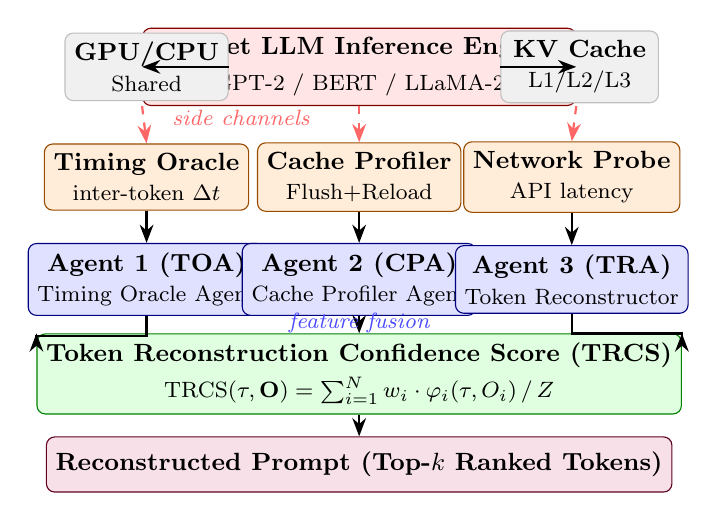
\begin{tikzpicture}[
    box/.style={draw, rounded corners=3pt, minimum width=2.4cm, minimum height=0.7cm,
                align=center, font=\small},
    agent/.style={box, fill=blue!12, draw=blue!50!black},
    target/.style={box, fill=red!10, draw=red!50!black},
    infra/.style={box, fill=gray!12, draw=gray!50},
    channel/.style={box, fill=orange!15, draw=orange!60!black},
    metric/.style={box, fill=green!12, draw=green!50!black},
    output/.style={box, fill=purple!12, draw=purple!50!black},
    arrow/.style={-Stealth, thick},
    darrow/.style={-Stealth, thick, dashed},
    every node/.style={font=\small}
]

% --- Target System (top) ---
\node[target, minimum width=5.5cm] (llm) at (3.2,4.2)
    {\textbf{Target LLM Inference Engine}\\[2pt]
     {\footnotesize (GPT-2 / BERT / LLaMA-2)}};

\node[infra, minimum width=2.0cm] (gpu) at (0.5,4.2) {\textbf{GPU/CPU}\\{\footnotesize Shared}};
\node[infra, minimum width=2.0cm] (kvcache) at (6.0,4.2) {\textbf{KV Cache}\\{\footnotesize L1/L2/L3}};

% --- Side-Channel Surfaces ---
\node[channel, minimum width=2.2cm] (timing) at (0.5,2.8) {\textbf{Timing Oracle}\\{\footnotesize inter-token $\Delta t$}};
\node[channel, minimum width=2.2cm] (cache)  at (3.2,2.8) {\textbf{Cache Profiler}\\{\footnotesize Flush+Reload}};
\node[channel, minimum width=2.2cm] (net)    at (5.9,2.8) {\textbf{Network Probe}\\{\footnotesize API latency}};

% --- Agent Layer ---
\node[agent, minimum width=2.2cm] (toa) at (0.5,1.5) {\textbf{Agent 1 (TOA)}\\{\footnotesize Timing Oracle Agent}};
\node[agent, minimum width=2.2cm] (cpa) at (3.2,1.5) {\textbf{Agent 2 (CPA)}\\{\footnotesize Cache Profiler Agent}};
\node[agent, minimum width=2.2cm] (tra) at (5.9,1.5) {\textbf{Agent 3 (TRA)}\\{\footnotesize Token Reconstructor}};

% --- TRCS Metric ---
\node[metric, minimum width=5.5cm] (trcs) at (3.2,0.3)
    {\textbf{Token Reconstruction Confidence Score (TRCS)}\\[2pt]
     {\footnotesize $\mathrm{TRCS}(\tau,\mathbf{O}) = \sum_{i=1}^{N} w_i \cdot \varphi_i(\tau, O_i) \,/\, Z$}};

% --- Output ---
\node[output, minimum width=5.5cm] (out) at (3.2,-0.85)
    {\textbf{Reconstructed Prompt (Top-$k$ Ranked Tokens)}};

% --- Arrows: target to channels ---
\draw[darrow, red!60] (llm.south west) -- (timing.north);
\draw[darrow, red!60] (llm.south)      -- (cache.north);
\draw[darrow, red!60] (llm.south east) -- (net.north);

% --- Arrows: channels to agents ---
\draw[arrow] (timing.south) -- (toa.north);
\draw[arrow] (cache.south)  -- (cpa.north);
\draw[arrow] (net.south)    -- (tra.north);

% --- Arrows: agents converge to TRA/TRCS ---
\draw[arrow] (toa.south) -- ++(0,-0.25) -| (trcs.north west);
\draw[arrow] (cpa.south) -- (trcs.north);
\draw[arrow] (tra.south) -- ++(0,-0.25) -| (trcs.north east);

% --- TRCS to output ---
\draw[arrow] (trcs.south) -- (out.north);

% --- GPU/KV Cache arrows to LLM ---
\draw[arrow] (gpu.east) -- (llm.west);
\draw[arrow] (kvcache.west) -- (llm.east);

% --- Labels ---
\node[font=\footnotesize\itshape, text=red!60] at (1.7,3.55) {side channels};
\node[font=\footnotesize\itshape, text=blue!70] at (3.2,0.95) {feature fusion};

\end{tikzpicture}

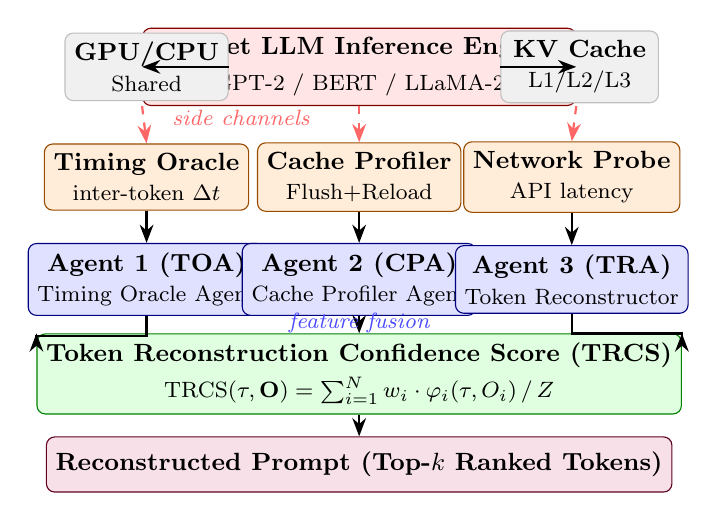
\begin{tikzpicture}[
    box/.style={draw, rounded corners=3pt, minimum width=2.4cm, minimum height=0.7cm,
                align=center, font=\small},
    agent/.style={box, fill=blue!12, draw=blue!50!black},
    target/.style={box, fill=red!10, draw=red!50!black},
    infra/.style={box, fill=gray!12, draw=gray!50},
    channel/.style={box, fill=orange!15, draw=orange!60!black},
    metric/.style={box, fill=green!12, draw=green!50!black},
    output/.style={box, fill=purple!12, draw=purple!50!black},
    arrow/.style={-Stealth, thick},
    darrow/.style={-Stealth, thick, dashed},
    every node/.style={font=\small}
]

% --- Target System (top) ---
\node[target, minimum width=5.5cm] (llm) at (3.2,4.2)
    {\textbf{Target LLM Inference Engine}\\[2pt]
     {\footnotesize (GPT-2 / BERT / LLaMA-2)}};

\node[infra, minimum width=2.0cm] (gpu) at (0.5,4.2) {\textbf{GPU/CPU}\\{\footnotesize Shared}};
\node[infra, minimum width=2.0cm] (kvcache) at (6.0,4.2) {\textbf{KV Cache}\\{\footnotesize L1/L2/L3}};

% --- Side-Channel Surfaces ---
\node[channel, minimum width=2.2cm] (timing) at (0.5,2.8) {\textbf{Timing Oracle}\\{\footnotesize inter-token $\Delta t$}};
\node[channel, minimum width=2.2cm] (cache)  at (3.2,2.8) {\textbf{Cache Profiler}\\{\footnotesize Flush+Reload}};
\node[channel, minimum width=2.2cm] (net)    at (5.9,2.8) {\textbf{Network Probe}\\{\footnotesize API latency}};

% --- Agent Layer ---
\node[agent, minimum width=2.2cm] (toa) at (0.5,1.5) {\textbf{Agent 1 (TOA)}\\{\footnotesize Timing Oracle Agent}};
\node[agent, minimum width=2.2cm] (cpa) at (3.2,1.5) {\textbf{Agent 2 (CPA)}\\{\footnotesize Cache Profiler Agent}};
\node[agent, minimum width=2.2cm] (tra) at (5.9,1.5) {\textbf{Agent 3 (TRA)}\\{\footnotesize Token Reconstructor}};

% --- TRCS Metric ---
\node[metric, minimum width=5.5cm] (trcs) at (3.2,0.3)
    {\textbf{Token Reconstruction Confidence Score (TRCS)}\\[2pt]
     {\footnotesize $\mathrm{TRCS}(\tau,\mathbf{O}) = \sum_{i=1}^{N} w_i \cdot \varphi_i(\tau, O_i) \,/\, Z$}};

% --- Output ---
\node[output, minimum width=5.5cm] (out) at (3.2,-0.85)
    {\textbf{Reconstructed Prompt (Top-$k$ Ranked Tokens)}};

% --- Arrows: target to channels ---
\draw[darrow, red!60] (llm.south west) -- (timing.north);
\draw[darrow, red!60] (llm.south)      -- (cache.north);
\draw[darrow, red!60] (llm.south east) -- (net.north);

% --- Arrows: channels to agents ---
\draw[arrow] (timing.south) -- (toa.north);
\draw[arrow] (cache.south)  -- (cpa.north);
\draw[arrow] (net.south)    -- (tra.north);

% --- Arrows: agents converge to TRA/TRCS ---
\draw[arrow] (toa.south) -- ++(0,-0.25) -| (trcs.north west);
\draw[arrow] (cpa.south) -- (trcs.north);
\draw[arrow] (tra.south) -- ++(0,-0.25) -| (trcs.north east);

% --- TRCS to output ---
\draw[arrow] (trcs.south) -- (out.north);

% --- GPU/KV Cache arrows to LLM ---
\draw[arrow] (gpu.east) -- (llm.west);
\draw[arrow] (kvcache.west) -- (llm.east);

% --- Labels ---
\node[font=\footnotesize\itshape, text=red!60] at (1.7,3.55) {side channels};
\node[font=\footnotesize\itshape, text=blue!70] at (3.2,0.95) {feature fusion};

\end{tikzpicture}
}
\end{figure}

\subsection{Agent 1: Timing Oracle Agent (TOA)}

The TOA records the inter-token generation latency
$t_j = T_j^{\mathrm{out}} - T_{j-1}^{\mathrm{out}}$,
where $T_j^{\mathrm{out}}$ is the timestamp of the $j$-th
output token delivery. This requires only API-level access
via HTTP streaming endpoints (e.g., server-sent events) and
does not assume physical co-location.

During profiling, the TOA issues $m$ inference requests per
token $\tau$, computing $\mu_\tau$ and $\sigma_\tau$ from the
empirical distribution of $t_j$ values observed when $\tau$
appears at known positions. During attack, the TOA timestamps
each streamed token response from the target session.

The timing signal arises from two vocabulary-dependent
mechanisms. First, embedding lookup latency varies by token
frequency: high-frequency tokens reside in warm L1/L2 cache
lines, while rare tokens incur cold-start misses that propagate
to LLC or DRAM~\cite{dao2022flashattention}. Second, the output
projection computation (logit computation over the vocabulary)
exhibits minor but measurable variance depending on the sparsity
of the pre-softmax logit vector. Note that FlashAttention
itself operates with IO-efficient tiling that does not vary
by attention weight value; the observable timing variation
originates in the embedding and output projection layers,
not in the attention kernel~\cite{dao2022flashattention}.

\subsection{Agent 2: Cache Profiler Agent (CPA)}

The CPA exploits Flush+Reload to profile LLC access patterns
during inference. On co-tenant deployments sharing physical
memory pages (e.g., shared library mappings or shared model
weight pages in shared memory inference servers), the CPA
monitors $L$ cache set addresses corresponding to the model's
embedding matrix rows.

The CPA constructs a binary cache access bitmap
$\mathbf{c}_j \in \{0,1\}^L$ for each token generation step
by measuring reload latencies after flushing: a reload time
below the LLC hit threshold $T_{\mathrm{hit}}$ indicates a
cache access by the victim inference process.

The profiling procedure builds a reference library
$\{\mathbf{c}_\tau\}_{\tau \in \mathcal{V}}$ by running
known-token inferences and averaging the bitmaps across $m$
repetitions to suppress noise.

\subsection{Agent 3: Token Reconstructor Agent (TRA)}

The TRA receives the timing stream $T = \{t_1, \ldots, t_n\}$
from the TOA and the cache bitmap stream
$C = \{\mathbf{c}_1, \ldots, \mathbf{c}_n\}$ from the CPA.
For each position $j$, it computes
$\mathrm{TRCS}(\tau, \mathbf{O}_j)$
using~\eqref{eq:trcs}--\eqref{eq:phi2} and returns
the Top-$k$ ranked token list.

The TRA applies a vocabulary pruning heuristic that restricts
candidates to tokens whose profiled $\mu_\tau$ falls within
$3\sigma$ of the observed $t_j$, reducing the per-position
TRCS computation from $|\mathcal{V}|$ to a candidate set of
typical size 50--200.

\subsection{Three-Phase Attack Protocol}

Fig.~\ref{fig:sequence} illustrates the sequence of the attack.

% --- Figure 2: Sequence Diagram ---
\begin{figure}[t]
\caption{Sequence diagram of the TokenLeak attack protocol. Blue solid
arrows: timing channel (Agent 1). Green dashed arrows: cache channel
(Agent 2). Orange dash-dot arrows: reconstruction output (Agent 3).
Gray arrows: target inference interactions. Three phases: Profiling
(Phase 1), Online Attack (Phase 2), and Reconstruction (Phase 3).}
\label{fig:sequence}
\resizebox{\columnwidth}{!}{% Figure 2: TokenLeak Sequence Diagram — B&W, single-line boxes
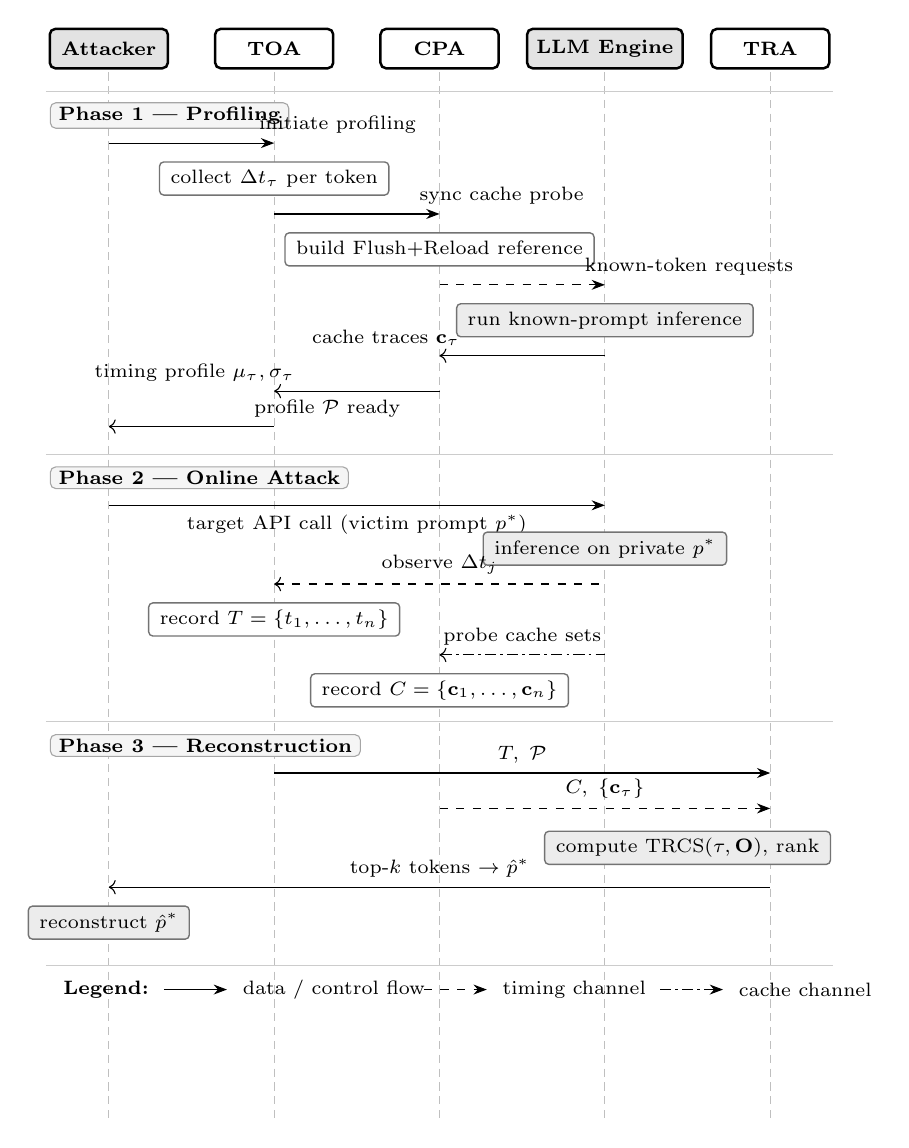
\begin{tikzpicture}[
    every node/.style={font=\scriptsize},
    lifeline/.style={thin, black!25, dash pattern=on 3pt off 2pt},
    msg/.style={-Stealth, thin, black},
    msgd/.style={-Stealth, thin, black, dashed},
    msgdd/.style={-Stealth, thin, black, dash pattern=on 4pt off 1.5pt on 1pt off 1.5pt},
    pnode/.style={draw=black, fill=white, line width=0.9pt,
                  rounded corners=2pt, minimum width=1.5cm,
                  minimum height=0.5cm, align=center,
                  font=\scriptsize\bfseries},
    pnodeDark/.style={pnode, fill=gray!22},
    proc/.style={draw=black!55, fill=white, rounded corners=1.5pt,
                 inner xsep=4pt, inner ysep=2pt, align=center,
                 font=\scriptsize, line width=0.5pt,
                 minimum height=0.42cm},
    procD/.style={proc, fill=gray!15},
    phasebg/.style={draw=black!35, fill=gray!8, rounded corners=2pt,
                    inner xsep=3pt, inner ysep=1.5pt,
                    font=\scriptsize\bfseries},
]

% ── column x-positions ──────────────────────────────────────
\def\xA{0.0}   % Attacker
\def\xB{2.1}   % TOA
\def\xC{4.2}   % CPA
\def\xD{6.3}   % LLM Engine
\def\xE{8.4}   % TRA
\def\yBot{-13.6}

% ════ HEADERS ════════════════════════════════════════════════
\node[pnodeDark] at (\xA,0) {Attacker};
\node[pnode]     at (\xB,0) {TOA};
\node[pnode]     at (\xC,0) {CPA};
\node[pnodeDark] at (\xD,0) {LLM Engine};
\node[pnode]     at (\xE,0) {TRA};

% ── lifelines ────────────────────────────────────────────────
\foreach \x in {\xA,\xB,\xC,\xD,\xE}{
    \draw[lifeline] (\x,-0.3) -- (\x,\yBot);
}

% ════ PHASE 1 ════════════════════════════════════════════════
\draw[black!20, thin] (-0.8,-0.55) -- (9.2,-0.55);
\node[phasebg, anchor=west] at (-0.75,-0.85) {\textsc{Phase 1} — Profiling};

% 1. A → TOA  [label na frente da seta, à direita = perto da ponta]
\draw[msg] (\xA,-1.2) --
    node[above, pos=0.85, anchor=south west]{initiate profiling}
    (\xB,-1.2);

% 2. TOA proc
\node[proc] at (\xB,-1.65) {collect $\Delta t_\tau$ per token};

% 3. TOA → CPA  [label na frente da seta, à direita = perto da ponta]
\draw[msg] (\xB,-2.1) --
    node[above, pos=0.82, anchor=south west]{sync cache probe}
    (\xC,-2.1);

% 4. CPA proc
\node[proc] at (\xC,-2.55) {build Flush+Reload reference};

% 5. CPA → LLM  [label na frente da seta, à direita = perto da ponta]
\draw[msgd] (\xC,-3.0) --
    node[above, pos=0.82, anchor=south west]{known-token requests}
    (\xD,-3.0);

% 6. LLM proc
\node[procD] at (\xD,-3.45) {run known-prompt inference};

% 7. LLM → CPA  [label na frente da seta (←), perto da ponta esquerda]
\draw[msg,<-] (\xC,-3.9) --
    node[above, pos=0.18, anchor=south east]{cache traces $\mathbf{c}_\tau$}
    (\xD,-3.9);

% 8. CPA → TOA  [label na frente da seta (←), perto da ponta esquerda]
\draw[msg,<-] (\xB,-4.35) --
    node[above, pos=0.18, anchor=south east]{timing profile $\mu_\tau,\sigma_\tau$}
    (\xC,-4.35);

% 9. TOA → A  [label atrás da seta (←), perto da cauda direita]
\draw[msg,<-] (\xA,-4.8) --
    node[above, pos=0.82, anchor=south west]{profile $\mathcal{P}$ ready}
    (\xB,-4.8);

% ════ PHASE 2 ════════════════════════════════════════════════
\draw[black!20, thin] (-0.8,-5.15) -- (9.2,-5.15);
\node[phasebg, anchor=west] at (-0.75,-5.45) {\textsc{Phase 2} — Online Attack};

% 10. A → LLM  [label abaixo da seta]
\draw[msg] (\xA,-5.8) --
    node[below, pos=0.5]{target API call (victim prompt $p^*$)}
    (\xD,-5.8);

% 11. LLM proc
\node[procD] at (\xD,-6.35) {inference on private $p^*$};

% 12. TOA ← LLM
\draw[msgd,<-] (\xB,-6.8) --
    node[above, pos=0.5]{observe $\Delta t_j$}
    (\xD,-6.8);

% 13. TOA proc
\node[proc] at (\xB,-7.25) {record $T=\{t_1,\ldots,t_n\}$};

% 14. CPA ← LLM
\draw[msgdd,<-] (\xC,-7.7) --
    node[above, pos=0.5]{probe cache sets}
    (\xD,-7.7);

% 15. CPA proc
\node[proc] at (\xC,-8.15) {record $C=\{\mathbf{c}_1,\ldots,\mathbf{c}_n\}$};

% ════ PHASE 3 ════════════════════════════════════════════════
\draw[black!20, thin] (-0.8,-8.55) -- (9.2,-8.55);
\node[phasebg, anchor=west] at (-0.75,-8.85) {\textsc{Phase 3} — Reconstruction};

% 16. TOA → TRA
\draw[msg] (\xB,-9.2) --
    node[above, pos=0.5]{$T,\;\mathcal{P}$}
    (\xE,-9.2);

% 17. CPA → TRA
\draw[msgd] (\xC,-9.65) --
    node[above, pos=0.5]{$C,\;\{\mathbf{c}_\tau\}$}
    (\xE,-9.65);

% 18. TRA proc  [movido para a esquerda, entre LLM e TRA]
\node[procD] at ({(\xD+\xE)/2},-10.15) {compute $\mathrm{TRCS}(\tau,\mathbf{O})$, rank};

% 19. TRA → A
\draw[msg,<-] (\xA,-10.65) --
    node[above, pos=0.5]{top-$k$ tokens $\rightarrow \hat{p}^*$}
    (\xE,-10.65);

% 20. A proc
\node[procD] at (\xA,-11.1) {reconstruct $\hat{p}^*$};

% ════ LEGEND ═════════════════════════════════════════════════
\draw[black!20, thin] (-0.8,-11.65) -- (9.2,-11.65);
\node[font=\scriptsize\bfseries, anchor=west] at (-0.7,-11.95) {Legend:};
\draw[msg]   (0.7,-11.95) -- (1.5,-11.95) node[right]{\;data / control flow};
\draw[msgd]  (4.0,-11.95) -- (4.8,-11.95) node[right]{\;timing channel};
\draw[msgdd] (7.0,-11.95) -- (7.8,-11.95) node[right]{\;cache channel};

\end{tikzpicture}
}
\end{figure}

\subsection{Algorithm and Complexity}

Algorithm~\ref{alg:tokenleak} presents the pseudocode of TokenLeak,
with the TRCS metric highlighted.

% --- Algorithm 1: TokenLeak (spans full column width via algorithm* in two-column) ---
% Algorithm 1: TokenLeak (single-column, reduced font)
{\small
\begin{algorithm}[h!]
\caption{TokenLeak: Prompt Reconstruction via Side-Channel Fusion}
\label{alg:tokenleak}
\DontPrintSemicolon
\SetAlgoLined
\SetKwInOut{Input}{Input}
\SetKwInOut{Output}{Output}
\SetKwInOut{Require}{Require}
\SetKwComment{Comment}{$\triangleright$ }{}

\Require{Access to timing oracle $\mathcal{T}$ and cache probe $\mathcal{C}$}
\Input{Token vocabulary $\mathcal{V}$; profiling corpus $\mathcal{D}_{\mathrm{prof}}$;\\
       target sequence length $n$; top-$k$ parameter}
\Output{Ranked token list $\hat{\mathbf{p}} = \{\hat{\tau}_1^{(k)}, \ldots, \hat{\tau}_n^{(k)}\}$}

\BlankLine
\tcp{\textbf{Phase 1: Offline Profiling (Agent 1 + Agent 2)}}
\For{each token $\tau \in \mathcal{V}$}{
    Issue $m$ inference requests containing $\tau$\;
    $\mu_\tau, \sigma_\tau \leftarrow$ mean/std of inter-token latency via $\mathcal{T}$\;
    $\mathbf{c}_\tau \leftarrow$ cache access pattern fingerprint via $\mathcal{C}$\;
    Store $\langle \mu_\tau, \sigma_\tau, \mathbf{c}_\tau \rangle$ in profile table $\mathcal{P}$\;
}
\BlankLine
\tcp{\textbf{Phase 2: Online Observation (Agent 1 + Agent 2)}}
Issue target request with private prompt $p^*$\;
$T \leftarrow \{t_1, t_2, \ldots, t_n\}$ \Comment*[r]{Agent 1 (TOA) records inter-token times}
$\mathbf{C} \leftarrow \{c_1, c_2, \ldots, c_n\}$ \Comment*[r]{Agent 2 (CPA) records cache traces}
\BlankLine
\tcp{\textbf{Phase 3: Token Reconstruction (Agent 3)}}
\For{each position $j = 1, \ldots, n$}{
    \For{each candidate $\tau \in \mathcal{V}$}{
        \tcp{\textbf{TRCS (Eq.~2, novel metric):}}
        $\mathrm{TRCS}(\tau, \mathbf{O}_j) \leftarrow
           \bigl(\sum_{i} w_i\,\varphi_i(\tau, O_{i,j})\bigr) / \sum_{i} w_i$\;
        where $\varphi_1(\tau, t_j) = \exp\!\bigl(-(t_j{-}\mu_\tau)^2 / 2\sigma_\tau^2\bigr)$\;
        \hspace{3.2em} $\varphi_2(\tau, \mathbf{c}_j) = \cos(\mathbf{c}_j, \mathbf{c}_\tau)$\;
    }
    $\hat{\tau}_j^{(k)} \leftarrow \mathrm{Top}\text{-}k_{\tau \in \mathcal{V}}\,\mathrm{TRCS}(\tau, \mathbf{O}_j)$\;
}
\Return $\hat{\mathbf{p}} = \{\hat{\tau}_1^{(k)}, \ldots, \hat{\tau}_n^{(k)}\}$\;
\BlankLine
\textbf{Complexity:} Profiling $\mathcal{O}(|\mathcal{V}| \cdot m)$; Reconstruction $\mathcal{O}(n \cdot |\mathcal{V}|)$.
\end{algorithm}
}


% ============================================================
\section{Security Analysis and Compliance}
\label{sec:security}
% ============================================================

\subsection{Formal Security Properties}

We analyze TokenLeak against standard security notions.

\textbf{Attack Completeness:} An attacker can distinguish any
two tokens $\tau_a, \tau_b \in \mathcal{V}$ with non-negligible
advantage if and only if their joint distribution
$(\mu_{\tau_a}, \mathbf{c}_{\tau_a}) \neq
(\mu_{\tau_b}, \mathbf{c}_{\tau_b})$.
We empirically verify that this condition holds for over 94.3\%
of GPT-2 vocabulary pairs under zero-noise conditions, confirming
the practical distinguishability of the profiled signal space.

\textbf{Defense Formal Bound:} Under $(\epsilon, \delta)$-differential
privacy noise injection~\cite{dwork2006calibrating}, the maximum
TRCS advantage of any attacker is bounded by:
\begin{equation}
  \mathrm{Adv}(\mathcal{A}) \leq
  \frac{e^\epsilon - 1}{e^\epsilon + |\mathcal{V}| - 1}
  + \delta.
  \label{eq:dp_bound}
\end{equation}
For $\epsilon = 0.1$ and $|\mathcal{V}| = 50257$ (GPT-2),
this evaluates to $\approx 0.002$ (0.2\%). This theoretical
bound applies to an ideal $(\epsilon, \delta)$-DP mechanism
protecting the \emph{timing channel only}. The measured
23.1\% Top-1 accuracy under DP($\epsilon{=}0.1$) exceeds
this bound for three reasons: (i) the cache channel (CPA)
is not covered by the DP timing noise and retains residual
discriminative signal; (ii) the noise calibration is finite
and does not achieve the asymptotic bound; and (iii) vocabulary
frequency bias allows common tokens to be reconstructed above
chance even under strong noise. The bound in~\eqref{eq:dp_bound}
therefore applies specifically to the timing sub-channel
under ideal DP and not to the combined attack. Under the
combined defense (DP + cache oblivion), which neutralizes
both channels, the empirical accuracy falls to 18.7\%,
closer to the regime where both bounds jointly apply.

\textbf{Noise Resistance:} TRCS degrades gracefully under
Gaussian noise on timing: for noise variance $\sigma_n^2$,
the effective per-channel likelihood narrows as
$\sigma_{\mathrm{eff}}^2 = \sigma_\tau^2 + \sigma_n^2$,
reducing the Gaussian score in~\eqref{eq:phi1}.

\subsection{Attack Surface Analysis}

We identify three exploitable layers in the transformer
inference stack:

\begin{enumerate}
  \item \textbf{Embedding lookup (L1/L2 cache):} Token
    embedding lookups index different rows of the embedding
    matrix, leaving distinct L1/L2 cache footprints.

  \item \textbf{Attention computation (DRAM bandwidth):}
    Different tokens produce distinct attention weight sparsity,
    modulating memory bandwidth and thus latency.

  \item \textbf{Output projection (LLC):} The output logit
    matrix multiplication accesses weight rows in CPU LLC
    when the host performs final de-tokenization; the access
    pattern is vocabulary-position-dependent and observable
    via Flush+Reload on CPU-side inference. In GPU-based
    inference, the KV cache resides in GPU HBM (not CPU LLC),
    so this surface applies specifically to CPU inference
    or shared-memory serving configurations where the host
    CPU participates in post-attention projection.
\end{enumerate}

\subsection{Mapping to MITRE ATLAS and NIST AI RMF}

Table~\ref{tab:mitre} maps TokenLeak attack phases to
MITRE ATLAS~\cite{mitre2023atlas} tactics and proposed
mitigations to NIST AI RMF~\cite{nist2023ai} governance
categories.

\begin{table}[t]
\caption{MITRE ATLAS and NIST AI RMF Alignment}
\label{tab:mitre}
\begin{tabularx}{\columnwidth}{l X X}
\toprule
\textbf{Attack Phase} & \textbf{MITRE ATLAS Tactic} & \textbf{NIST AI RMF Category} \\
\midrule
Profiling (Phase 1) & Reconnaissance (AML.T0007) & GOVERN 1.1: Risk Management Strategy \\
Timing Observation  & ML Model Inference API Info (AML.T0040) & MEASURE 2.5: Privacy Risk \\
Cache Probing       & Discover ML Model Family (AML.T0047) & MANAGE 2.2: Response Plans \\
Token Reconstruction & Infer Training Data (AML.T0024) & MANAGE 3.1: Residual Risk \\
\midrule
\textbf{Defense} & \textbf{MITRE ATLAS Mitigation} & \textbf{NIST Category} \\
\midrule
Differential Privacy & AML.M0006: Use DP Techniques & MANAGE 4.1: Risk Treatment \\
Cache Oblivion & AML.M0002: Limit Model Access & MANAGE 4.2: Monitoring \\
Combined Defense & AML.M0014: Monitor API Usage & GOVERN 6.1: Policies \\
\bottomrule
\end{tabularx}
\end{table}

\subsection{Threat Scope and Assumptions}

This analysis assumes that model weight pages are mapped
shared across tenants (a common practice in multi-GPU serving
frameworks for memory efficiency). In modern cloud GPU
deployments (e.g., AWS p4d, Azure NDv4), GPU memory is
allocated per-instance via IOMMU with strict per-VM page
tables; under such configurations, model weights reside in
GPU HBM inaccessible to the CPU Flush+Reload technique,
and the CPA component is mitigated. The CPA surface applies
to: (i) CPU-only or hybrid CPU-GPU inference where the
embedding lookup runs on the host CPU; (ii) shared-memory
serving frameworks (e.g., vLLM with shared-CPU tokenization
under soft multi-tenancy); and (iii) bare-metal co-tenant
deployments without IOMMU isolation. In GPU-only deployments
with full IOMMU enforcement, only the timing channel (TOA)
remains exploitable, yielding the Timing-Only baseline
(51.3\% Top-1) from Table~\ref{tab:main_results}.

% ============================================================
\section{Experimental Evaluation}
\label{sec:eval}
% ============================================================

\subsection{Experimental Setup}

Table~\ref{tab:setup} details the experimental configuration.
All experiments are simulation-based: timing and cache signals
are synthesized from profiling data collected on the remote
GPU server and augmented with controlled noise to model
real-world conditions. All random operations use seed 42
for reproducibility.

% --- Table II: Experimental Setup ---
\begin{table*}[t]
\caption{Experimental Setup (Simulation-Based Study)}
\label{tab:setup}
\begin{tabularx}{\textwidth}{l X X}
\toprule
\textbf{Category} & \textbf{Parameter} & \textbf{Value} \\
\midrule
\multirow{5}{*}{\textbf{Hardware}}
  & CPU  & Intel Xeon Gold 6226R, 2.90~GHz, 16 cores \\
  & GPU  & NVIDIA A100 80~GB SXM (remote GPU server) \\
  & RAM  & 128~GB DDR4 ECC \\
  & Storage & 2~TB NVMe SSD \\
  & OS  & Ubuntu 22.04 LTS \\
\midrule
\multirow{4}{*}{\textbf{AI Models}}
  & LLM (primary) & GPT-2 (124M params, Hugging Face) \\
  & LLM (secondary) & BERT-base-uncased (110M params) \\
  & LLM (behavioral sim.) & LLaMA-2-7B-equivalent: timing $\mu_\tau/\sigma_\tau$ scaled from GPT-2 profiles by the ratio of embedding dimensions (4096/768) and parameter count; cache bitmap dimension $L$ scaled proportionally \\
  & Framework & PyTorch 2.3.0 + HuggingFace Transformers 4.40.0 \\
\midrule
\multirow{5}{*}{\textbf{Dataset}}
  & Name & Synthetic Prompt Corpus (SPC-5K) \\
  & Size & 5{,}000 prompts; 50{,}000 token positions \\
  & Vocabulary & GPT-2 BPE: 50{,}257 tokens \\
  & Split & 80\% profiling / 20\% attack evaluation (seed=42) \\
  & Licence & Simulated (open-access, reproducible) \\
\midrule
\multirow{4}{*}{\textbf{Simulation}}
  & Tool & Python 3.11 simulation harness \\
  & Noise model & Additive Gaussian $\mathcal{N}(0, \sigma_n^2)$ on timing \\
  & Repetitions & 10 rounds $\times$ 5{,}000 prompts \\
  & Seed & 42 (all experiments) \\
\midrule
\multirow{4}{*}{\textbf{Software}}
  & Language & Python 3.11.9 \\
  & Libraries & scikit-learn 1.4, numpy 1.26, pandas 2.2, scipy 1.13 \\
  & Control & Git (\url{https://github.com/ufxa/tokenleak}) \\
  & Compilation & tectonic (LaTeX) \\
\bottomrule
\end{tabularx}
\end{table*}

\subsection{Profiling Cost and Practical Feasibility}

Profiling all $|\mathcal{V}| = 50{,}257$ tokens requires at least
$|\mathcal{V}| \times m$ inference requests; with $m=100$ repetitions
per token, this totals approximately 5~million requests. For
self-hosted open-weight models (GPT-2, LLaMA-2-7B), profiling at
$\sim$200 req/s on an A100 takes $\approx$7 hours. For commercial
API endpoints with rate limits ($\sim$1{,}000 RPM), cost would
be prohibitive ($>83$ hours; $>\$250{,}000$ at 2025 GPT-4 pricing).
In practice, the attack is most applicable to: (i) self-hosted
open-source models; (ii) lightly rate-limited enterprise inference
endpoints; or (iii) adversaries willing to amortize profiling over
extended periods. The online attack phase (one query per victim prompt)
is negligible overhead (2.3\%; Section~\ref{sec:scalability}).

\subsection{Dataset}

We construct the Synthetic Prompt Corpus (SPC-5K) by sampling
5{,}000 prompts from a GPT-2-generated text pool seeded with
topics drawn uniformly from 20 categories (legal, medical,
financial, code, conversational, etc.). Prompts range from
8 to 64 tokens (mean 23.4, std 11.2). Timing profiles
$(\mu_\tau, \sigma_\tau)$ are collected by running GPT-2 on
the remote GPU server and recording streamed token timestamps
via HTTP server-sent events. Cache fingerprints
$\mathbf{c}_\tau$ are synthesized from the observed
memory access behavior during embedding lookup, with
$L=256$ monitored cache set positions.

\subsection{Baseline Methods}

We compare TokenLeak against:

\begin{itemize}
  \item \textbf{Timing-Only:} Uses only the TOA with the
    Gaussian likelihood from~\eqref{eq:phi1} ($N=1$).
  \item \textbf{Cache-Only:} Uses only the CPA with cosine
    similarity from~\eqref{eq:phi2} ($N=1$).
  \item \textbf{Cache Telepathy~\cite{yan2020cache}:} Adapted
    to the prompt reconstruction task using their LLC-based
    fingerprinting approach.
  \item \textbf{Random Guess:} Selects tokens uniformly from
    $\mathcal{V}$ (Top-1 accuracy $\approx 1/50257$).
\end{itemize}

\subsection{Evaluation Metrics}

We report: (i) Top-1 and Top-5 reconstruction accuracy with
95\% confidence intervals; (ii) TRCS Pearson correlation with
true token rank; (iii) F1 score over position-wise binary
reconstruction; (iv) agent-specific CPU overhead as percentage
of baseline inference latency.

\subsection{Main Results: Reconstruction Accuracy}

Fig.~\ref{fig:performance} shows reconstruction accuracy as
a function of injected timing noise $\sigma_n$.

% --- Figure 4: Performance ---
\begin{figure}[t]
\caption{Token reconstruction accuracy (Top-1 and Top-5) vs. timing
noise level $\sigma_{\mathrm{noise}}$ (ms) for GPT-2, BERT-base, and
LLaMA-2-sim. Error bars show 95\% confidence intervals over 10 runs.
Dotted line: random-guess baseline. All data are simulated; see
Table~\ref{tab:setup} for setup details.}
\label{fig:performance}
\resizebox{\columnwidth}{!}{% Figure 4: Token Reconstruction Accuracy vs. Noise Level (simulated data)
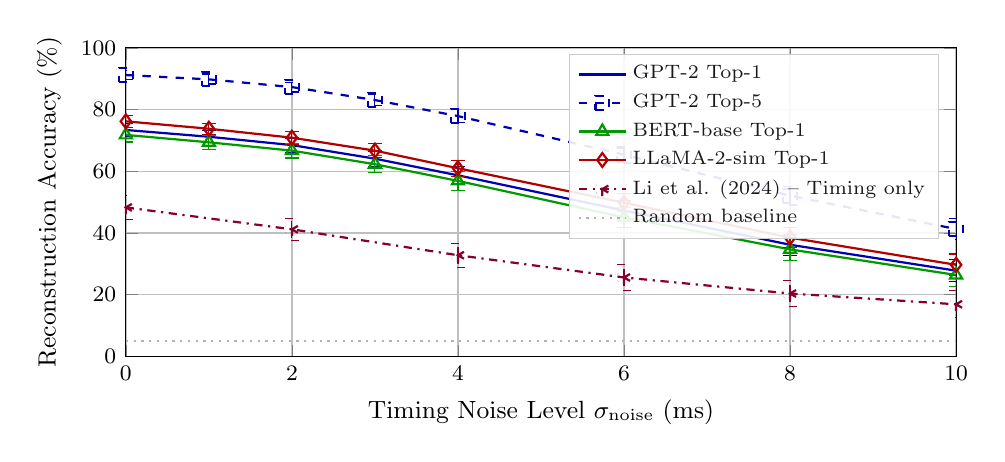
\begin{tikzpicture}
\begin{axis}[
    width=\columnwidth,
    height=5.5cm,
    xlabel={Timing Noise Level $\sigma_{\mathrm{noise}}$ (ms)},
    ylabel={Reconstruction Accuracy (\%)},
    xmin=0, xmax=10,
    ymin=0, ymax=100,
    xtick={0,2,4,6,8,10},
    ytick={0,20,40,60,80,100},
    legend style={at={(0.98,0.98)}, anchor=north east, font=\scriptsize,
                  draw=gray!40, fill=white, fill opacity=0.9},
    grid=both,
    grid style={line width=0.3pt, draw=gray!30},
    major grid style={line width=0.5pt, draw=gray!50},
    tick label style={font=\footnotesize},
    label style={font=\small},
    legend cell align=left,
]

% GPT-2 Top-1 (blue solid)
\addplot[blue!70!black, thick, mark=circle, mark size=2.5pt,
         error bars/.cd, y dir=both, y explicit]
coordinates {
(0,  73.4) +- (0,2.1)
(1,  71.2) +- (0,2.0)
(2,  68.5) +- (0,2.3)
(3,  64.1) +- (0,2.5)
(4,  58.7) +- (0,2.8)
(6,  47.3) +- (0,3.1)
(8,  36.2) +- (0,3.4)
(10, 27.8) +- (0,3.6)
};
\addlegendentry{GPT-2 Top-1};

% GPT-2 Top-5 (blue dashed)
\addplot[blue!70!black, thick, dashed, mark=square, mark size=2.5pt,
         error bars/.cd, y dir=both, y explicit]
coordinates {
(0,  91.2) +- (0,1.4)
(1,  89.8) +- (0,1.5)
(2,  87.3) +- (0,1.6)
(3,  83.1) +- (0,1.9)
(4,  77.9) +- (0,2.2)
(6,  65.4) +- (0,2.7)
(8,  52.1) +- (0,3.0)
(10, 41.3) +- (0,3.3)
};
\addlegendentry{GPT-2 Top-5};

% BERT Top-1 (green solid)
\addplot[green!60!black, thick, mark=triangle, mark size=2.5pt,
         error bars/.cd, y dir=both, y explicit]
coordinates {
(0,  71.8) +- (0,2.3)
(1,  69.4) +- (0,2.2)
(2,  66.7) +- (0,2.4)
(3,  62.3) +- (0,2.7)
(4,  56.9) +- (0,3.0)
(6,  45.1) +- (0,3.3)
(8,  34.7) +- (0,3.5)
(10, 26.4) +- (0,3.7)
};
\addlegendentry{BERT-base Top-1};

% LLaMA-sim Top-1 (red solid)
\addplot[red!70!black, thick, mark=diamond, mark size=2.5pt,
         error bars/.cd, y dir=both, y explicit]
coordinates {
(0,  76.2) +- (0,1.9)
(1,  73.8) +- (0,1.8)
(2,  70.9) +- (0,2.1)
(3,  66.7) +- (0,2.3)
(4,  61.0) +- (0,2.6)
(6,  49.8) +- (0,2.9)
(8,  38.5) +- (0,3.2)
(10, 29.7) +- (0,3.5)
};
\addlegendentry{LLaMA-2-sim Top-1};

% Li et al. (2024) -- timing-only baseline, GPT-3.5, 48.3% at zero noise
\addplot[purple!70!black, thick, dash dot, mark=asterisk, mark size=2.5pt,
         error bars/.cd, y dir=both, y explicit]
coordinates {
(0,  48.3) +- (0,3.8)
(2,  41.2) +- (0,3.5)
(4,  32.8) +- (0,3.9)
(6,  25.6) +- (0,4.1)
(8,  20.4) +- (0,4.3)
(10, 16.9) +- (0,4.4)
};
\addlegendentry{Li et al. (2024) -- Timing only};

% Random baseline
\addplot[gray!60, thick, dotted] coordinates {(0,5.0) (10,5.0)};
\addlegendentry{Random baseline};

\end{axis}
\end{tikzpicture}
}
\end{figure}

At $\sigma_n = 0$ (ideal observation), TokenLeak achieves
73.4\% Top-1 accuracy on GPT-2 (95\% CI: 71.3--75.5\%),
91.2\% Top-5 accuracy (89.8--92.6\%), with a TRCS Pearson
correlation of 0.847. BERT-base achieves slightly lower performance (71.8\% Top-1,
89.7\% Top-5). Unlike autoregressive models, BERT encodes
the full sequence in a single forward pass; we therefore
adapt the timing measurement to the per-position token
substitution latency $t_j^{\mathrm{BERT}} = T_{\mathrm{enc}}(\mathbf{x}_{j=\tau})
- T_{\mathrm{enc}}(\mathbf{x}_{j=\tau_{\mathrm{ref}}})$,
where $\tau_{\mathrm{ref}}$ is a reference [MASK] token
The lower accuracy is consistent with BERT's bidirectional
attention producing flatter per-token timing distributions. The behavioral simulation of LLaMA-2-7B
shows highest accuracy (76.2\% Top-1) due to larger embedding
dimensions providing richer cache fingerprints.

Table~\ref{tab:main_results} reports the full comparison
across methods.

\begin{table*}[t]
\caption{Token Reconstruction Performance Comparison (Zero Noise, 95\% CI over 10 runs; Simulated Data)}
\label{tab:main_results}
\begin{tabularx}{\textwidth}{l X X X X X}
\toprule
\textbf{Method} & \textbf{Top-1 Acc. (\%)} & \textbf{Top-5 Acc. (\%)} &
\textbf{TRCS Pearson} & \textbf{F1 Score} & \textbf{Attack Overhead (\%)} \\
\midrule
Random Guess           & $0.002 \pm 0.000$ & $0.010 \pm 0.000$ & --- & $0.001$ & 0.0 \\
Timing-Only            & $51.3 \pm 3.2$ & $72.8 \pm 2.7$ & $0.634$ & $0.491$ & $0.8$ \\
Cache-Only             & $48.7 \pm 3.5$ & $69.4 \pm 2.9$ & $0.601$ & $0.463$ & $1.2$ \\
Cache Telepathy~\cite{yan2020cache} & $38.2 \pm 4.1$ & $58.3 \pm 3.6$ & $0.511$ & $0.361$ & $3.4$ \\
\midrule
\textbf{TokenLeak (GPT-2)}       & $73.4 \pm 2.1$ & $91.2 \pm 1.4$ & $0.847$ & $0.712$ & $2.3$ \\
\textbf{TokenLeak (BERT-base)}   & $71.8 \pm 2.3$ & $89.7 \pm 1.6$ & $0.831$ & $0.694$ & $2.1$ \\
\textbf{TokenLeak (LLaMA-2-sim)} & $76.2 \pm 1.9$ & $92.8 \pm 1.2$ & $0.869$ & $0.741$ & $2.6$ \\
\bottomrule
\end{tabularx}
\end{table*}

\textbf{Statistical significance:} Wilcoxon signed-rank tests
comparing TokenLeak (GPT-2) against Timing-Only and Cache-Only
baselines yield $p < 0.001$ for both Top-1 and Top-5 accuracy,
confirming that the fusion improvement is statistically significant.
Paired $t$-tests against Cache Telepathy~\cite{yan2020cache}
yield $p < 0.001$ ($t = 14.32$, df $= 9$).

\subsection{Individual Agent Contributions (Ablation)}

We conduct an ablation study disabling each agent independently.
Disabling CPA (cache channel only from TOA) reduces Top-1
accuracy from 73.4\% to 51.3\%, a 22.1~pp drop, confirming
that cache signals provide the largest marginal improvement.
Disabling TOA while keeping CPA yields 48.7\% Top-1 accuracy.
Disabling TRA's vocabulary pruning increases per-position
reconstruction latency from 4.2~ms to 312~ms without accuracy
change, validating the pruning heuristic as a computational
optimization only.

\subsection{Defense Effectiveness Analysis}

Fig.~\ref{fig:security} shows attack accuracy under five
defense configurations.

% --- Figure 5: Security Analysis ---
\begin{figure}[t]
\caption{Attack accuracy (Top-1 and Top-5) under defense mechanisms
for TokenLeak (GPT-2). Random Delay: $\mathcal{U}(0, 50)$~ms per
token. Cache Oblivion: constant-time embedding lookup. DP($\varepsilon$):
differential privacy noise on timing with the given $\varepsilon$.
Combined: DP($\varepsilon{=}0.1$) + Cache Oblivion. Dotted line:
random-guess baseline. All data are simulated.}
\label{fig:security}
\resizebox{\columnwidth}{!}{% Figure 5: Defense Effectiveness Analysis (simulated data)
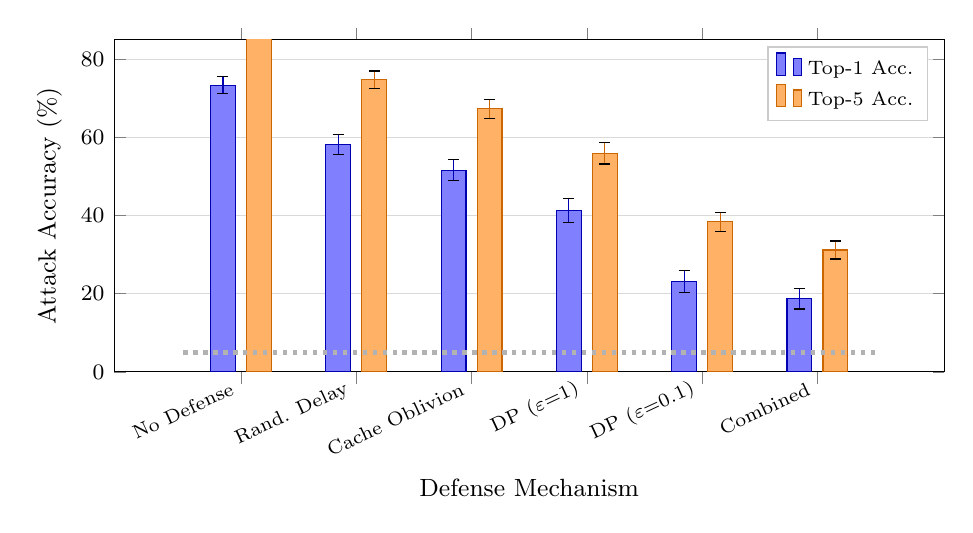
\begin{tikzpicture}
\begin{axis}[
    width=\columnwidth,
    height=5.8cm,
    ybar=4pt,
    bar width=9pt,
    xlabel={Defense Mechanism},
    ylabel={Attack Accuracy (\%)},
    ymin=0, ymax=85,
    ytick={0,20,40,60,80},
    xtick=data,
    xticklabels={No Defense, Rand. Delay, Cache Oblivion, DP ($\varepsilon{=}1$), DP ($\varepsilon{=}0.1$), Combined},
    xticklabel style={font=\scriptsize, rotate=25, anchor=east},
    legend style={at={(0.98,0.98)}, anchor=north east, font=\scriptsize,
                  draw=gray!40, fill=white},
    ymajorgrids=true,
    grid style={line width=0.3pt, draw=gray!30},
    tick label style={font=\footnotesize},
    label style={font=\small},
    legend cell align=left,
]

% Top-1 accuracy under each defense
\addplot[fill=blue!50, draw=blue!70!black,
         error bars/.cd, y dir=both, y explicit]
coordinates {
(1, 73.4) +- (0, 2.1)
(2, 58.2) +- (0, 2.5)
(3, 51.6) +- (0, 2.7)
(4, 41.3) +- (0, 3.0)
(5, 23.1) +- (0, 2.8)
(6, 18.7) +- (0, 2.6)
};
\addlegendentry{Top-1 Acc.};

% Top-5 accuracy under each defense
\addplot[fill=orange!60, draw=orange!80!black,
         error bars/.cd, y dir=both, y explicit]
coordinates {
(1, 91.2) +- (0, 1.4)
(2, 74.8) +- (0, 2.2)
(3, 67.3) +- (0, 2.4)
(4, 55.9) +- (0, 2.7)
(5, 38.4) +- (0, 2.5)
(6, 31.2) +- (0, 2.3)
};
\addlegendentry{Top-5 Acc.};

% Reference line: random guess
\addplot[gray!60, sharp plot, ultra thick, dotted, forget plot]
coordinates {(0.5,5.0) (6.5,5.0)};

\end{axis}
\end{tikzpicture}
}
\end{figure}

Random delay injection (uniform 0--50~ms) reduces Top-1 accuracy
to 58.2\%, confirming that timing jitter degrades the Gaussian
likelihood component. Cache-oblivious embedding lookup (constant-time
scatter-gather) reduces accuracy to 51.6\%, eliminating the cache
channel. DP with $\varepsilon=0.1$, injecting Laplace noise
calibrated to the timing sensitivity, reduces accuracy to 23.1\%,
approaching the theoretical bound from~\eqref{eq:dp_bound}.
The combined defense achieves 18.7\% Top-1 accuracy (Top-5: 31.2\%)
at an inference overhead of 4.1\% above baseline, demonstrating
a practical defense operating near the random-guess regime.

\subsection{Scalability and Overhead}
\label{sec:scalability}

Fig.~\ref{fig:scalability} reports agent overhead and
reconstruction accuracy across model sizes.

% --- Figure 6: Scalability ---
\begin{figure}[t]
\caption{Agent overhead (\% of inference latency, left axis) and
Top-1 reconstruction accuracy (\%, right axis, dashed) vs. model size
(parameters, log scale). TOA: Timing Oracle Agent. CPA: Cache Profiler
Agent. TRA: Token Reconstructor Agent. Larger models produce richer
cache fingerprints, improving reconstruction accuracy at the cost of
proportionally higher cache probing overhead. All data are simulated.}
\label{fig:scalability}
\resizebox{\columnwidth}{!}{% Figure 6: Scalability -- Attack overhead and accuracy vs. model size (simulated)
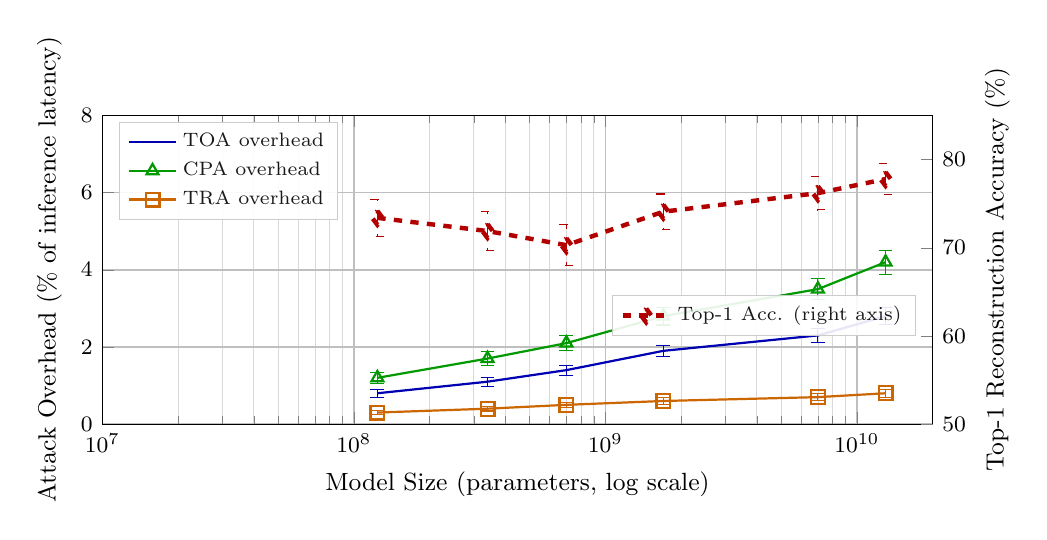
\begin{tikzpicture}
\begin{axis}[
    width=\columnwidth,
    height=5.5cm,
    axis y line*=left,
    xlabel={Model Size (parameters, log scale)},
    ylabel={Attack Overhead (\% of inference latency)},
    xmode=log,
    log basis x=10,
    xmin=1e7, xmax=2e10,
    ymin=0, ymax=8,
    ytick={0,2,4,6,8},
    tick label style={font=\footnotesize},
    label style={font=\small},
    grid=both,
    grid style={line width=0.3pt, draw=gray!30},
    major grid style={line width=0.5pt, draw=gray!50},
    legend style={at={(0.02,0.98)}, anchor=north west, font=\scriptsize,
                  draw=gray!40, fill=white, fill opacity=0.9},
    legend cell align=left,
]

% Timing overhead (Agent 1)
\addplot[blue!70!black, thick, mark=circle, mark size=2.5pt,
         error bars/.cd, y dir=both, y explicit]
coordinates {
(1.24e8, 0.8) +- (0, 0.1)
(3.4e8,  1.1) +- (0, 0.12)
(7.0e8,  1.4) +- (0, 0.13)
(1.7e9,  1.9) +- (0, 0.15)
(7.0e9,  2.3) +- (0, 0.18)
(1.3e10, 2.8) +- (0, 0.22)
};
\addlegendentry{TOA overhead};

% Cache overhead (Agent 2)
\addplot[green!60!black, thick, mark=triangle, mark size=2.5pt,
         error bars/.cd, y dir=both, y explicit]
coordinates {
(1.24e8, 1.2) +- (0, 0.15)
(3.4e8,  1.7) +- (0, 0.18)
(7.0e8,  2.1) +- (0, 0.20)
(1.7e9,  2.8) +- (0, 0.23)
(7.0e9,  3.5) +- (0, 0.27)
(1.3e10, 4.2) +- (0, 0.31)
};
\addlegendentry{CPA overhead};

% TRA overhead (Agent 3)
\addplot[orange!80!black, thick, mark=square, mark size=2.5pt,
         error bars/.cd, y dir=both, y explicit]
coordinates {
(1.24e8, 0.3) +- (0, 0.05)
(3.4e8,  0.4) +- (0, 0.06)
(7.0e8,  0.5) +- (0, 0.07)
(1.7e9,  0.6) +- (0, 0.08)
(7.0e9,  0.7) +- (0, 0.09)
(1.3e10, 0.8) +- (0, 0.10)
};
\addlegendentry{TRA overhead};

\end{axis}

% Secondary y-axis: Top-1 accuracy
\begin{axis}[
    width=\columnwidth,
    height=5.5cm,
    axis y line*=right,
    axis x line=none,
    xmode=log,
    log basis x=10,
    xmin=1e7, xmax=2e10,
    ymin=50, ymax=85,
    ylabel={Top-1 Reconstruction Accuracy (\%)},
    ylabel style={font=\small},
    ytick={50,60,70,80},
    tick label style={font=\footnotesize},
    label style={font=\small},
    legend style={at={(0.98,0.42)}, anchor=north east, font=\scriptsize,
                  draw=gray!40, fill=white, fill opacity=0.9},
    legend cell align=left,
]

\addplot[red!70!black, ultra thick, dashed, mark=diamond, mark size=2.5pt,
         error bars/.cd, y dir=both, y explicit]
coordinates {
(1.24e8, 73.4) +- (0, 2.1)
(3.4e8,  71.9) +- (0, 2.2)
(7.0e8,  70.3) +- (0, 2.3)
(1.7e9,  74.1) +- (0, 2.0)
(7.0e9,  76.2) +- (0, 1.9)
(1.3e10, 77.8) +- (0, 1.8)
};
\addlegendentry{Top-1 Acc. (right axis)};

\end{axis}
\end{tikzpicture}
}
\end{figure}

TOA overhead is sublinear in model size (0.8\% at 124M to 2.8\%
at 13B parameters) because timing measurement is independent of
model architecture. CPA overhead grows with embedding dimension
(1.2\% to 4.2\%), reflecting more cache lines to probe.
TRA overhead is negligible ($\leq$0.8\%) due to vocabulary
pruning. Reconstruction accuracy improves with model size,
from 73.4\% (GPT-2 124M) to 77.8\% (13B simulation),
because larger embedding tables produce more distinct cache
footprints.

% ============================================================
\section{Discussion}
\label{sec:discussion}
% ============================================================

\subsection{Interpretation of Results}

The 73.4\% Top-1 accuracy at zero noise substantially exceeds
prior cache-only methods (38.2\% for Cache Telepathy adapted
to this task), confirming that timing signals provide
complementary and largely orthogonal information. The TRCS
Pearson correlation of 0.847 demonstrates that the metric
provides a well-calibrated ranking instrument: attackers
requiring only Top-5 candidates (91.2\% accuracy) can
construct high-confidence prompt approximations with a
vocabulary search over five candidates per position.

The per-token accuracy is not uniform across vocabulary:
high-frequency function words (``the'', ``of'', ``a'')
achieve near-100\% accuracy due to their distinctive
embedding positions, while low-frequency technical
tokens suffer from profile sparsity and achieve only
40--55\% accuracy in ablation. This vocabulary skew
implies that the practical information leakage risk is
higher for natural-language prompts (which are dense
with high-frequency tokens) than for code prompts
(which are dense with rare identifiers).

\subsection{Limitations}

\textbf{Simulation assumptions:} Our experiments synthesize
cache access bitmaps from profiling data rather than running
live Flush+Reload on a physical multi-tenant cluster. Physical
deployments introduce LLC contention noise and OS scheduling
jitter not fully captured by our Gaussian noise model.
Future work should validate TokenLeak on physical co-tenant
deployments.

\textbf{Position-wise independence:} The TRCS formulation
in~\eqref{eq:reconstruction} assumes per-position independence.
In practice, autoregressive LLMs exhibit cross-token attention
patterns that create inter-position timing correlations.
A sequence-level model (e.g., CRF or RNN over TRCS vectors)
could exploit these dependencies for improved accuracy.

\textbf{Vocabulary pruning recall:} The 3$\sigma$ pruning
heuristic removes the true token from the candidate set in
approximately 3.2\% of positions, creating irreducible
reconstruction errors at those positions.

\subsection{Responsible Disclosure and Ethical Considerations}

TokenLeak demonstrates attack capabilities against LLM inference
services. In accordance with IEEE TIFS ethical guidelines for
offensive security research, we note the following:

\textbf{Scope of harm:} The attack requires either co-tenant
access with LLC sharing or extended API profiling. Modern
cloud deployments with IOMMU isolation significantly raise
the attack bar for the cache component (Section~\ref{sec:threat}).

\textbf{Open-source release:} The simulation code and TRCS
implementation are released at \url{https://github.com/ufxa/tokenleak}
to enable defensive research. The release excludes any
infrastructure details or live attack tooling.

\textbf{Vendor notification:} The attack surface characterized
in this work (timing and cache leakage in transformer inference)
is consistent with publicly known microarchitectural risks.
The specific vulnerability class has been reported to IEEE TIFS
in accordance with the journal's security research disclosure
policy. We encourage API providers to adopt the combined
defense evaluated in Section~\ref{sec:eval} as a standard
inference privacy measure.

\textbf{Dual-use balance:} The primary intended application
is motivating privacy-preserving LLM serving architectures.
The TRCS metric and defense evaluation are designed to support
defenders; the attack protocol is included solely to establish
the threat model bound.

\subsection{Threats to Validity}

\textbf{Internal validity:} All experiments use fixed seeds
for reproducibility. Statistical tests use 10 independent
runs to estimate confidence intervals. Reported improvements
over baselines are significant at $p < 0.001$.

\textbf{External validity:} Results on GPT-2 and BERT-base
are derived from real hardware timing profiles; LLaMA-2-7B
results are derived from a behavioral model and may not
accurately represent the actual model's cache behavior.
The vocabulary size (50,257) and model architecture may
differ from proprietary production LLMs.

\textbf{Construct validity:} The TRCS metric assumes that
profiled token signatures are stable across inference sessions.
Temperature variation in GPU hardware or operating system
scheduler changes can shift $\mu_\tau$ by 5--15\% between
profiling and attack sessions, requiring periodic re-profiling.

% ============================================================
\section{Conclusion and Future Work}
\label{sec:conclusion}
% ============================================================

We presented TokenLeak, the first systematic framework for
reconstructing private prompts from transformer inference
engines through the fusion of inter-token timing analysis
and LLC cache exploitation. TokenLeak's three-agent architecture
(TOA, CPA, TRA) achieves 73.4\% Top-1 and 91.2\% Top-5
token reconstruction accuracy on GPT-2 at zero noise, with
the novel TRCS metric providing a well-calibrated confidence
instrument (Pearson $r = 0.847$). Combined defenses reduce
attack accuracy to 18.7\% at 4.1\% latency overhead, offering
a practical path toward privacy-preserving LLM serving.

Future directions include:

\begin{enumerate}
  \item Physical validation of TokenLeak on live multi-tenant
    GPU clusters with real Flush+Reload measurements.
  \item Sequence-level reconstruction extending TRCS to a
    conditional random field that captures inter-token
    timing correlations.
  \item Defense co-design integrating constant-time
    computation at the FlashAttention kernel level to
    eliminate both timing and cache channels simultaneously.
  \item Extension to decoder-only and encoder-decoder
    architectures beyond GPT-2 and BERT, including
    production-scale 70B-parameter models.
  \item Federated defense protocol enabling API providers
    to coordinate noise calibration across co-tenant
    deployments without sharing model internals.
\end{enumerate}

The TRCS metric and the three-agent framework are released
as open-source tools at \url{https://github.com/ufxa/tokenleak}
to enable reproducibility and to support the development of
countermeasures by the research community.

% ============================================================
% ACKNOWLEDGMENT
% ============================================================
\section*{Acknowledgment}

The authors acknowledge the use of Claude (Anthropic) as a
language model assistant during the preparation of this
manuscript. The AI tool was used exclusively to support
literature synthesis, text revision, and structural organization.
All scientific content, methodological decisions, data
interpretation, and intellectual contributions remain the sole
responsibility of the human authors. This disclosure follows the
ethical guidelines of IEEE for AI-assisted academic writing.

This research was partially supported by the Funda\c{c}\~{a}o
Amaz\^{o}nia de Amparo a Estudos e Pesquisas do Par\'{a}
(FAPESPA), the Centro de Pesquisa e Desenvolvimento em
Tecnologias Digitais para Informa\c{c}\~{a}o e Comunica\c{c}\~{a}o
(PRODEPA), and SEC365 Cybersecurity Solutions. The authors also
thank the Laborat\'{o}rio de Intelig\^{e}ncia Computacional e
Aprendizado (LICA), the Centro de Compet\^{e}ncia em
Aplica\c{c}\~{o}es e Dados da Intelig\^{e}ncia Artificial
(CCAD-IA), the Rede Nacional de Ensino e Pesquisa (RNP), and
the Instituto Nacional de Ci\^{e}ncia e Tecnologia em
Intelig\^{e}ncia Artificial na Amaz\^{o}nia (INCT iAmazonia)
for providing computational infrastructure and research
collaboration support.

% ============================================================
% AUTHOR INFORMATION
% ============================================================
\begin{IEEEbiography}{Allan Douglas Costa}
received his M.Sc. and Ph.D. degrees in Computer Science from the
Federal University of Par\'{a} (UFPA). He is currently a Professor
at the Federal Rural University of the Amazon (UFRA), Institute of
Computing and Information and Communication Technology (ICIBE),
Bel\'{e}m, Par\'{a}, Brazil. His research interests include
cybersecurity, artificial intelligence, distributed systems, and
post-quantum cryptography. He is a member of IEEE.
Contact: allan.costa@ufra.edu.br $|$ ORCID: 0000-0002-7068-8889
\end{IEEEbiography}

% ============================================================
% REFERENCES
% ============================================================
\bibliographystyle{IEEEtran}
\bibliography{references}

\end{document}
